\documentclass[1p]{elsarticle_modified}
%\bibliographystyle{elsarticle-num}

%\usepackage[colorlinks]{hyperref}
%\usepackage{abbrmath_seonhwa} %\Abb, \Ascr, \Acal ,\Abf, \Afrak
\usepackage{amsfonts}
\usepackage{amssymb}
\usepackage{amsmath}
\usepackage{amsthm}
\usepackage{scalefnt}
\usepackage{amsbsy}
\usepackage{kotex}
\usepackage{caption}
\usepackage{subfig}
\usepackage{color}
\usepackage{graphicx}
\usepackage{xcolor} %% white, black, red, green, blue, cyan, magenta, yellow
\usepackage{float}
\usepackage{setspace}
\usepackage{hyperref}

\usepackage{tikz}
\usetikzlibrary{arrows}

\usepackage{multirow}
\usepackage{array} % fixed length table
\usepackage{hhline}

%%%%%%%%%%%%%%%%%%%%%
\makeatletter
\renewcommand*\env@matrix[1][\arraystretch]{%
	\edef\arraystretch{#1}%
	\hskip -\arraycolsep
	\let\@ifnextchar\new@ifnextchar
	\array{*\c@MaxMatrixCols c}}
\makeatother %https://tex.stackexchange.com/questions/14071/how-can-i-increase-the-line-spacing-in-a-matrix
%%%%%%%%%%%%%%%

\usepackage[normalem]{ulem}

\newcommand{\msout}[1]{\ifmmode\text{\sout{\ensuremath{#1}}}\else\sout{#1}\fi}
%SOURCE: \msout is \stkout macro in https://tex.stackexchange.com/questions/20609/strikeout-in-math-mode

\newcommand{\cancel}[1]{
	\ifmmode
	{\color{red}\msout{#1}}
	\else
	{\color{red}\sout{#1}}
	\fi
}

\newcommand{\add}[1]{
	{\color{blue}\uwave{#1}}
}

\newcommand{\replace}[2]{
	\ifmmode
	{\color{red}\msout{#1}}{\color{blue}\uwave{#2}}
	\else
	{\color{red}\sout{#1}}{\color{blue}\uwave{#2}}
	\fi
}

\newcommand{\Sol}{\mathcal{S}} %segment
\newcommand{\D}{D} %diagram
\newcommand{\A}{\mathcal{A}} %arc


%%%%%%%%%%%%%%%%%%%%%%%%%%%%%5 test

\def\sl{\operatorname{\textup{SL}}(2,\Cbb)}
\def\psl{\operatorname{\textup{PSL}}(2,\Cbb)}
\def\quan{\mkern 1mu \triangleright \mkern 1mu}

\theoremstyle{definition}
\newtheorem{thm}{Theorem}[section]
\newtheorem{prop}[thm]{Proposition}
\newtheorem{lem}[thm]{Lemma}
\newtheorem{ques}[thm]{Question}
\newtheorem{cor}[thm]{Corollary}
\newtheorem{defn}[thm]{Definition}
\newtheorem{exam}[thm]{Example}
\newtheorem{rmk}[thm]{Remark}
\newtheorem{alg}[thm]{Algorithm}

\newcommand{\I}{\sqrt{-1}}
\begin{document}

%\begin{frontmatter}
%
%\title{Boundary parabolic representations of knots up to 8 crossings}
%
%%% Group authors per affiliation:
%\author{Yunhi Cho} 
%\address{Department of Mathematics, University of Seoul, Seoul, Korea}
%\ead{yhcho@uos.ac.kr}
%
%
%\author{Seonhwa Kim} %\fnref{s_kim}}
%\address{Center for Geometry and Physics, Institute for Basic Science, Pohang, 37673, Korea}
%\ead{ryeona17@ibs.re.kr}
%
%\author{Hyuk Kim}
%\address{Department of Mathematical Sciences, Seoul National University, Seoul 08826, Korea}
%\ead{hyukkim@snu.ac.kr}
%
%\author{Seokbeom Yoon}
%\address{Department of Mathematical Sciences, Seoul National University, Seoul, 08826,  Korea}
%\ead{sbyoon15@snu.ac.kr}
%
%\begin{abstract}
%We find all boundary parabolic representation of knots up to 8 crossings.
%
%\end{abstract}
%\begin{keyword}
%    \MSC[2010] 57M25 
%\end{keyword}
%
%\end{frontmatter}

%\linenumbers
%\tableofcontents
%
\newcommand\colored[1]{\textcolor{white}{\rule[-0.35ex]{0.8em}{1.4ex}}\kern-0.8em\color{red} #1}%
%\newcommand\colored[1]{\textcolor{white}{ #1}\kern-2.17ex	\textcolor{white}{ #1}\kern-1.81ex	\textcolor{white}{ #1}\kern-2.15ex\color{red}#1	}

{\Large $\underline{12a_{0595}~(K12a_{0595})}$}

\setlength{\tabcolsep}{10pt}
\renewcommand{\arraystretch}{1.6}
\vspace{1cm}\begin{tabular}{m{100pt}>{\centering\arraybackslash}m{274pt}}
\multirow{5}{120pt}{
	\centering
	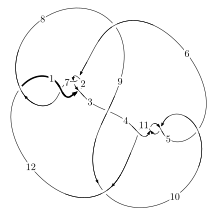
\includegraphics[width=112pt]{../../../GIT/diagram.site/Diagrams/png/1396_12a_0595.png}\\
\ \ \ A knot diagram\footnotemark}&
\allowdisplaybreaks
\textbf{Linearized knot diagam} \\
\cline{2-2}
 &
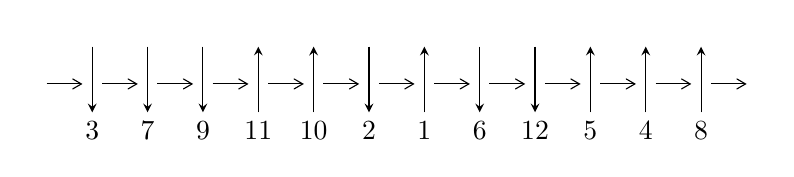
\begin{tikzpicture}[x=20pt, y=17pt]
	% nodes
	\node (C0) at (0, 0) {};
	\node (C1) at (1, 0) {};
	\node (C1U) at (1, +1) {};
	\node (C1D) at (1, -1) {3};

	\node (C2) at (2, 0) {};
	\node (C2U) at (2, +1) {};
	\node (C2D) at (2, -1) {7};

	\node (C3) at (3, 0) {};
	\node (C3U) at (3, +1) {};
	\node (C3D) at (3, -1) {9};

	\node (C4) at (4, 0) {};
	\node (C4U) at (4, +1) {};
	\node (C4D) at (4, -1) {11};

	\node (C5) at (5, 0) {};
	\node (C5U) at (5, +1) {};
	\node (C5D) at (5, -1) {10};

	\node (C6) at (6, 0) {};
	\node (C6U) at (6, +1) {};
	\node (C6D) at (6, -1) {2};

	\node (C7) at (7, 0) {};
	\node (C7U) at (7, +1) {};
	\node (C7D) at (7, -1) {1};

	\node (C8) at (8, 0) {};
	\node (C8U) at (8, +1) {};
	\node (C8D) at (8, -1) {6};

	\node (C9) at (9, 0) {};
	\node (C9U) at (9, +1) {};
	\node (C9D) at (9, -1) {12};

	\node (C10) at (10, 0) {};
	\node (C10U) at (10, +1) {};
	\node (C10D) at (10, -1) {5};

	\node (C11) at (11, 0) {};
	\node (C11U) at (11, +1) {};
	\node (C11D) at (11, -1) {4};

	\node (C12) at (12, 0) {};
	\node (C12U) at (12, +1) {};
	\node (C12D) at (12, -1) {8};
	\node (C13) at (13, 0) {};

	% arrows
	\draw[->,>={angle 60}]
	(C0) edge (C1) (C1) edge (C2) (C2) edge (C3) (C3) edge (C4) (C4) edge (C5) (C5) edge (C6) (C6) edge (C7) (C7) edge (C8) (C8) edge (C9) (C9) edge (C10) (C10) edge (C11) (C11) edge (C12) (C12) edge (C13) ;	\draw[->,>=stealth]
	(C1U) edge (C1D) (C2U) edge (C2D) (C3U) edge (C3D) (C4D) edge (C4U) (C5D) edge (C5U) (C6U) edge (C6D) (C7D) edge (C7U) (C8U) edge (C8D) (C9U) edge (C9D) (C10D) edge (C10U) (C11D) edge (C11U) (C12D) edge (C12U) ;
	\end{tikzpicture} \\
\hhline{~~} \\& 
\textbf{Solving Sequence} \\ \cline{2-2} 
 &
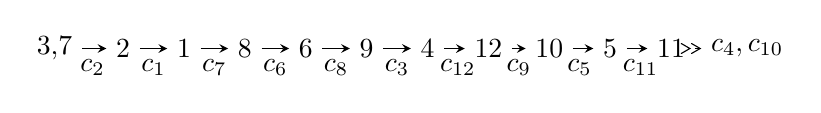
\begin{tikzpicture}[x=22pt, y=7pt]
	% node
	\node (A0) at (-1/8, 0) {3,7};
	\node (A1) at (1, 0) {2};
	\node (A2) at (2, 0) {1};
	\node (A3) at (3, 0) {8};
	\node (A4) at (4, 0) {6};
	\node (A5) at (5, 0) {9};
	\node (A6) at (6, 0) {4};
	\node (A7) at (7, 0) {12};
	\node (A8) at (8, 0) {10};
	\node (A9) at (9, 0) {5};
	\node (A10) at (10, 0) {11};
	\node (C1) at (1/2, -1) {$c_{2}$};
	\node (C2) at (3/2, -1) {$c_{1}$};
	\node (C3) at (5/2, -1) {$c_{7}$};
	\node (C4) at (7/2, -1) {$c_{6}$};
	\node (C5) at (9/2, -1) {$c_{8}$};
	\node (C6) at (11/2, -1) {$c_{3}$};
	\node (C7) at (13/2, -1) {$c_{12}$};
	\node (C8) at (15/2, -1) {$c_{9}$};
	\node (C9) at (17/2, -1) {$c_{5}$};
	\node (C10) at (19/2, -1) {$c_{11}$};
	\node (A11) at (45/4, 0) {$c_{4},c_{10}$};

	% edge
	\draw[->,>=stealth]	
	(A0) edge (A1) (A1) edge (A2) (A2) edge (A3) (A3) edge (A4) (A4) edge (A5) (A5) edge (A6) (A6) edge (A7) (A7) edge (A8) (A8) edge (A9) (A9) edge (A10) ;
	\draw[->>,>={angle 60}]	
	(A10) edge (A11);
\end{tikzpicture} \\ 

\end{tabular} \\

\footnotetext{
The image of knot diagram is generated by the software ``\textbf{Draw programme}" developed by Andrew Bartholomew(\url{http://www.layer8.co.uk/maths/draw/index.htm\#Running-draw}), where we modified some parts for our purpose(\url{https://github.com/CATsTAILs/LinksPainter}).
}\phantom \\ \newline 
\centering \textbf{Ideals for irreducible components\footnotemark of $X_{\text{par}}$} 
 
\begin{align*}
I^u_{1}&=\langle 
u^{69}+u^{68}+\cdots- u-1\rangle \\
\\
\end{align*}
\raggedright * 1 irreducible components of $\dim_{\mathbb{C}}=0$, with total 69 representations.\\
\footnotetext{All coefficients of polynomials are rational numbers. But the coefficients are sometimes approximated in decimal forms when there is not enough margin.}
\newpage
\renewcommand{\arraystretch}{1}
\centering \section*{I. $I^u_{1}= \langle u^{69}+u^{68}+\cdots- u-1 \rangle$}
\flushleft \textbf{(i) Arc colorings}\\
\begin{tabular}{m{7pt} m{180pt} m{7pt} m{180pt} }
\flushright $a_{3}=$&$\begin{pmatrix}1\\0\end{pmatrix}$ \\
\flushright $a_{7}=$&$\begin{pmatrix}0\\u\end{pmatrix}$ \\
\flushright $a_{2}=$&$\begin{pmatrix}1\\- u^2\end{pmatrix}$ \\
\flushright $a_{1}=$&$\begin{pmatrix}- u^2+1\\- u^2\end{pmatrix}$ \\
\flushright $a_{8}=$&$\begin{pmatrix}u^5-2 u^3+u\\u^5- u^3+u\end{pmatrix}$ \\
\flushright $a_{6}=$&$\begin{pmatrix}u\\- u^3+u\end{pmatrix}$ \\
\flushright $a_{9}=$&$\begin{pmatrix}- u^9+2 u^7- u^5-2 u^3+u\\u^{11}-3 u^9+4 u^7- u^5- u^3+u\end{pmatrix}$ \\
\flushright $a_{4}=$&$\begin{pmatrix}- u^{20}+5 u^{18}-11 u^{16}+10 u^{14}+2 u^{12}-13 u^{10}+9 u^8-3 u^4+u^2+1\\u^{22}-6 u^{20}+17 u^{18}-26 u^{16}+20 u^{14}-13 u^{10}+10 u^8- u^6-2 u^4+u^2\end{pmatrix}$ \\
\flushright $a_{12}=$&$\begin{pmatrix}- u^8+3 u^6-3 u^4+1\\- u^8+2 u^6-2 u^4\end{pmatrix}$ \\
\flushright $a_{10}=$&$\begin{pmatrix}- u^{27}+8 u^{25}+\cdots+4 u^5- u^3\\- u^{27}+7 u^{25}+\cdots- u^3+u\end{pmatrix}$ \\
\flushright $a_{5}=$&$\begin{pmatrix}u^{57}-16 u^{55}+\cdots- u^5+u\\u^{57}-15 u^{55}+\cdots- u^5+u\end{pmatrix}$ \\
\flushright $a_{11}=$&$\begin{pmatrix}u^{50}-13 u^{48}+\cdots+u^2+1\\- u^{52}+14 u^{50}+\cdots-6 u^8- u^4\end{pmatrix}$\\&\end{tabular}
\flushleft \textbf{(ii) Obstruction class $= -1$}\\~\\
\flushleft \textbf{(iii) Cusp Shapes $= -4 u^{67}+72 u^{65}+\cdots-8 u^3+2$}\\~\\
\newpage\renewcommand{\arraystretch}{1}
\flushleft \textbf{(iv) u-Polynomials at the component}\newline \\
\begin{tabular}{m{50pt}|m{274pt}}
Crossings & \hspace{64pt}u-Polynomials at each crossing \\
\hline $$\begin{aligned}c_{1}\end{aligned}$$&$\begin{aligned}
&u^{69}+37 u^{68}+\cdots- u+1
\end{aligned}$\\
\hline $$\begin{aligned}c_{2},c_{6}\end{aligned}$$&$\begin{aligned}
&u^{69}- u^{68}+\cdots- u+1
\end{aligned}$\\
\hline $$\begin{aligned}c_{3}\end{aligned}$$&$\begin{aligned}
&u^{69}- u^{68}+\cdots-4205 u+841
\end{aligned}$\\
\hline $$\begin{aligned}c_{4},c_{5},c_{10}\\c_{11}\end{aligned}$$&$\begin{aligned}
&u^{69}- u^{68}+\cdots- u+1
\end{aligned}$\\
\hline $$\begin{aligned}c_{7},c_{12}\end{aligned}$$&$\begin{aligned}
&u^{69}-3 u^{68}+\cdots+u+1
\end{aligned}$\\
\hline $$\begin{aligned}c_{8}\end{aligned}$$&$\begin{aligned}
&u^{69}-9 u^{68}+\cdots-183 u+13
\end{aligned}$\\
\hline $$\begin{aligned}c_{9}\end{aligned}$$&$\begin{aligned}
&u^{69}-19 u^{68}+\cdots+4845 u-283
\end{aligned}$\\
\hline
\end{tabular}\\~\\
\newpage\renewcommand{\arraystretch}{1}
\flushleft \textbf{(v) Riley Polynomials at the component}\newline \\
\begin{tabular}{m{50pt}|m{274pt}}
Crossings & \hspace{64pt}Riley Polynomials at each crossing \\
\hline $$\begin{aligned}c_{1}\end{aligned}$$&$\begin{aligned}
&y^{69}-9 y^{68}+\cdots+3 y-1
\end{aligned}$\\
\hline $$\begin{aligned}c_{2},c_{6}\end{aligned}$$&$\begin{aligned}
&y^{69}-37 y^{68}+\cdots- y-1
\end{aligned}$\\
\hline $$\begin{aligned}c_{3}\end{aligned}$$&$\begin{aligned}
&y^{69}-29 y^{68}+\cdots+24176227 y-707281
\end{aligned}$\\
\hline $$\begin{aligned}c_{4},c_{5},c_{10}\\c_{11}\end{aligned}$$&$\begin{aligned}
&y^{69}+79 y^{68}+\cdots- y-1
\end{aligned}$\\
\hline $$\begin{aligned}c_{7},c_{12}\end{aligned}$$&$\begin{aligned}
&y^{69}+55 y^{68}+\cdots-85 y-1
\end{aligned}$\\
\hline $$\begin{aligned}c_{8}\end{aligned}$$&$\begin{aligned}
&y^{69}-5 y^{68}+\cdots+1535 y-169
\end{aligned}$\\
\hline $$\begin{aligned}c_{9}\end{aligned}$$&$\begin{aligned}
&y^{69}-13 y^{68}+\cdots+1486623 y-80089
\end{aligned}$\\
\hline
\end{tabular}\\~\\
\newpage\flushleft \textbf{(vi) Complex Volumes and Cusp Shapes}
$$\begin{array}{c|c|c}  
\text{Solutions to }I^u_{1}& \I (\text{vol} + \sqrt{-1}CS) & \text{Cusp shape}\\
 \hline 
\begin{aligned}
u &= -1.007650 + 0.064350 I\end{aligned}
 & -3.60184 + 2.81733 I & -9.32476 - 5.48757 I \\ \hline\begin{aligned}
u &= -1.007650 - 0.064350 I\end{aligned}
 & -3.60184 - 2.81733 I & -9.32476 + 5.48757 I \\ \hline\begin{aligned}
u &= \phantom{-}0.863362 + 0.530746 I\end{aligned}
 & \phantom{-}0.35930 - 6.77991 I & -0.61658 + 10.23881 I \\ \hline\begin{aligned}
u &= \phantom{-}0.863362 - 0.530746 I\end{aligned}
 & \phantom{-}0.35930 + 6.77991 I & -0.61658 - 10.23881 I \\ \hline\begin{aligned}
u &= -0.835974 + 0.511530 I\end{aligned}
 & \phantom{-}1.64738 + 3.32051 I & \phantom{-}3.54071 - 4.43827 I \\ \hline\begin{aligned}
u &= -0.835974 - 0.511530 I\end{aligned}
 & \phantom{-}1.64738 - 3.32051 I & \phantom{-}3.54071 + 4.43827 I \\ \hline\begin{aligned}
u &= -0.879803 + 0.544272 I\end{aligned}
 & -7.29269 + 9.02370 I & -3.47414 - 8.26985 I \\ \hline\begin{aligned}
u &= -0.879803 - 0.544272 I\end{aligned}
 & -7.29269 - 9.02370 I & -3.47414 + 8.26985 I \\ \hline\begin{aligned}
u &= \phantom{-}0.859864 + 0.398364 I\end{aligned}
 & -1.45583 - 1.56617 I & -5.75209 + 2.95981 I \\ \hline\begin{aligned}
u &= \phantom{-}0.859864 - 0.398364 I\end{aligned}
 & -1.45583 + 1.56617 I & -5.75209 - 2.95981 I \\ \hline\begin{aligned}
u &= \phantom{-}1.050990 + 0.067740 I\end{aligned}
 & -11.48740 - 4.67055 I & -10.85743 + 3.45107 I \\ \hline\begin{aligned}
u &= \phantom{-}1.050990 - 0.067740 I\end{aligned}
 & -11.48740 + 4.67055 I & -10.85743 - 3.45107 I \\ \hline\begin{aligned}
u &= \phantom{-}0.763010 + 0.535883 I\end{aligned}
 & -3.25699 - 2.16890 I & \phantom{-}0.53836 + 3.82901 I \\ \hline\begin{aligned}
u &= \phantom{-}0.763010 - 0.535883 I\end{aligned}
 & -3.25699 + 2.16890 I & \phantom{-}0.53836 - 3.82901 I \\ \hline\begin{aligned}
u &= \phantom{-}0.931899\phantom{ +0.000000I}\end{aligned}
 & -1.68818\phantom{ +0.000000I} & -4.45100\phantom{ +0.000000I} \\ \hline\begin{aligned}
u &= -0.983730 + 0.422361 I\end{aligned}
 & -9.02531 + 0.64002 I & -6.52857 + 0. I\phantom{ +0.000000I} \\ \hline\begin{aligned}
u &= -0.983730 - 0.422361 I\end{aligned}
 & -9.02531 - 0.64002 I & -6.52857 + 0. I\phantom{ +0.000000I} \\ \hline\begin{aligned}
u &= -0.689201 + 0.500960 I\end{aligned}
 & \phantom{-}2.07105 + 0.85287 I & \phantom{-}5.34302 - 3.58736 I \\ \hline\begin{aligned}
u &= -0.689201 - 0.500960 I\end{aligned}
 & \phantom{-}2.07105 - 0.85287 I & \phantom{-}5.34302 + 3.58736 I \\ \hline\begin{aligned}
u &= -0.614253 + 0.561310 I\end{aligned}
 & -6.54819 - 4.59342 I & -1.49782 + 1.94707 I \\ \hline\begin{aligned}
u &= -0.614253 - 0.561310 I\end{aligned}
 & -6.54819 + 4.59342 I & -1.49782 - 1.94707 I \\ \hline\begin{aligned}
u &= \phantom{-}0.637725 + 0.530123 I\end{aligned}
 & \phantom{-}0.99322 + 2.46697 I & \phantom{-}1.50189 - 3.71848 I \\ \hline\begin{aligned}
u &= \phantom{-}0.637725 - 0.530123 I\end{aligned}
 & \phantom{-}0.99322 - 2.46697 I & \phantom{-}1.50189 + 3.71848 I \\ \hline\begin{aligned}
u &= -1.107000 + 0.388573 I\end{aligned}
 & -9.04626 + 0.50923 I & \phantom{-0.000000 } 0 \\ \hline\begin{aligned}
u &= -1.107000 - 0.388573 I\end{aligned}
 & -9.04626 - 0.50923 I & \phantom{-0.000000 } 0 \\ \hline\begin{aligned}
u &= -0.137752 + 0.815117 I\end{aligned}
 & -10.8743 - 9.4349 I & -5.12264 + 5.41104 I \\ \hline\begin{aligned}
u &= -0.137752 - 0.815117 I\end{aligned}
 & -10.8743 + 9.4349 I & -5.12264 - 5.41104 I \\ \hline\begin{aligned}
u &= \phantom{-}0.135322 + 0.801855 I\end{aligned}
 & -2.99570 + 7.10512 I & -2.78124 - 7.18886 I \\ \hline\begin{aligned}
u &= \phantom{-}0.135322 - 0.801855 I\end{aligned}
 & -2.99570 - 7.10512 I & -2.78124 + 7.18886 I \\ \hline\begin{aligned}
u &= -0.073813 + 0.807863 I\end{aligned}
 & -12.67980 + 0.44790 I & -7.20362 + 0.05375 I\\
 \hline 
 \end{array}$$\newpage$$\begin{array}{c|c|c}  
\text{Solutions to }I^u_{1}& \I (\text{vol} + \sqrt{-1}CS) & \text{Cusp shape}\\
 \hline 
\begin{aligned}
u &= -0.073813 - 0.807863 I\end{aligned}
 & -12.67980 - 0.44790 I & -7.20362 - 0.05375 I \\ \hline\begin{aligned}
u &= -0.127650 + 0.782006 I\end{aligned}
 & -1.37080 - 3.50950 I & \phantom{-}0.93203 + 2.31314 I \\ \hline\begin{aligned}
u &= -0.127650 - 0.782006 I\end{aligned}
 & -1.37080 + 3.50950 I & \phantom{-}0.93203 - 2.31314 I \\ \hline\begin{aligned}
u &= \phantom{-}0.087303 + 0.782586 I\end{aligned}
 & -4.38416 + 0.86576 I & -5.85927 + 0.77218 I \\ \hline\begin{aligned}
u &= \phantom{-}0.087303 - 0.782586 I\end{aligned}
 & -4.38416 - 0.86576 I & -5.85927 - 0.77218 I \\ \hline\begin{aligned}
u &= \phantom{-}1.127960 + 0.449076 I\end{aligned}
 & -2.38041 - 2.24656 I & \phantom{-0.000000 } 0 \\ \hline\begin{aligned}
u &= \phantom{-}1.127960 - 0.449076 I\end{aligned}
 & -2.38041 + 2.24656 I & \phantom{-0.000000 } 0 \\ \hline\begin{aligned}
u &= -1.142880 + 0.475125 I\end{aligned}
 & -2.14308 + 5.59560 I & \phantom{-0.000000 } 0 \\ \hline\begin{aligned}
u &= -1.142880 - 0.475125 I\end{aligned}
 & -2.14308 - 5.59560 I & \phantom{-0.000000 } 0 \\ \hline\begin{aligned}
u &= \phantom{-}1.153950 + 0.498640 I\end{aligned}
 & -8.24718 - 7.43164 I & \phantom{-0.000000 } 0 \\ \hline\begin{aligned}
u &= \phantom{-}1.153950 - 0.498640 I\end{aligned}
 & -8.24718 + 7.43164 I & \phantom{-0.000000 } 0 \\ \hline\begin{aligned}
u &= \phantom{-}1.199180 + 0.389997 I\end{aligned}
 & -5.28056 - 0.45902 I & \phantom{-0.000000 } 0 \\ \hline\begin{aligned}
u &= \phantom{-}1.199180 - 0.389997 I\end{aligned}
 & -5.28056 + 0.45902 I & \phantom{-0.000000 } 0 \\ \hline\begin{aligned}
u &= -1.209940 + 0.381438 I\end{aligned}
 & -7.02202 - 3.10940 I & \phantom{-0.000000 } 0 \\ \hline\begin{aligned}
u &= -1.209940 - 0.381438 I\end{aligned}
 & -7.02202 + 3.10940 I & \phantom{-0.000000 } 0 \\ \hline\begin{aligned}
u &= \phantom{-}0.183314 + 0.704841 I\end{aligned}
 & -5.44368 + 2.87522 I & -1.31258 - 3.07627 I \\ \hline\begin{aligned}
u &= \phantom{-}0.183314 - 0.704841 I\end{aligned}
 & -5.44368 - 2.87522 I & -1.31258 + 3.07627 I \\ \hline\begin{aligned}
u &= -1.205010 + 0.410064 I\end{aligned}
 & -8.18209 + 3.26828 I & \phantom{-0.000000 } 0 \\ \hline\begin{aligned}
u &= -1.205010 - 0.410064 I\end{aligned}
 & -8.18209 - 3.26828 I & \phantom{-0.000000 } 0 \\ \hline\begin{aligned}
u &= \phantom{-}1.218430 + 0.378071 I\end{aligned}
 & -14.9696 + 5.4032 I & \phantom{-0.000000 } 0 \\ \hline\begin{aligned}
u &= \phantom{-}1.218430 - 0.378071 I\end{aligned}
 & -14.9696 - 5.4032 I & \phantom{-0.000000 } 0 \\ \hline\begin{aligned}
u &= \phantom{-}1.218030 + 0.415989 I\end{aligned}
 & -16.5257 - 4.7100 I & \phantom{-0.000000 } 0 \\ \hline\begin{aligned}
u &= \phantom{-}1.218030 - 0.415989 I\end{aligned}
 & -16.5257 + 4.7100 I & \phantom{-0.000000 } 0 \\ \hline\begin{aligned}
u &= \phantom{-}1.194350 + 0.489511 I\end{aligned}
 & -7.61719 - 5.52009 I & \phantom{-0.000000 } 0 \\ \hline\begin{aligned}
u &= \phantom{-}1.194350 - 0.489511 I\end{aligned}
 & -7.61719 + 5.52009 I & \phantom{-0.000000 } 0 \\ \hline\begin{aligned}
u &= -1.188620 + 0.503633 I\end{aligned}
 & -4.47624 + 8.24964 I & \phantom{-0.000000 } 0 \\ \hline\begin{aligned}
u &= -1.188620 - 0.503633 I\end{aligned}
 & -4.47624 - 8.24964 I & \phantom{-0.000000 } 0 \\ \hline\begin{aligned}
u &= \phantom{-}1.193800 + 0.510098 I\end{aligned}
 & -6.11348 - 11.92620 I & \phantom{-0.000000 } 0 \\ \hline\begin{aligned}
u &= \phantom{-}1.193800 - 0.510098 I\end{aligned}
 & -6.11348 + 11.92620 I & \phantom{-0.000000 } 0 \\ \hline\begin{aligned}
u &= -1.206320 + 0.487082 I\end{aligned}
 & -16.0195 + 4.2556 I & \phantom{-0.000000 } 0\\
 \hline 
 \end{array}$$\newpage$$\begin{array}{c|c|c}  
\text{Solutions to }I^u_{1}& \I (\text{vol} + \sqrt{-1}CS) & \text{Cusp shape}\\
 \hline 
\begin{aligned}
u &= -1.206320 - 0.487082 I\end{aligned}
 & -16.0195 - 4.2556 I & \phantom{-0.000000 } 0 \\ \hline\begin{aligned}
u &= -1.198100 + 0.513816 I\end{aligned}
 & -14.0097 + 14.3072 I & \phantom{-0.000000 } 0 \\ \hline\begin{aligned}
u &= -1.198100 - 0.513816 I\end{aligned}
 & -14.0097 - 14.3072 I & \phantom{-0.000000 } 0 \\ \hline\begin{aligned}
u &= -0.386946 + 0.563275 I\end{aligned}
 & -7.28945 + 3.35761 I & -1.95583 - 2.56316 I \\ \hline\begin{aligned}
u &= -0.386946 - 0.563275 I\end{aligned}
 & -7.28945 - 3.35761 I & -1.95583 + 2.56316 I \\ \hline\begin{aligned}
u &= -0.163148 + 0.605619 I\end{aligned}
 & \phantom{-}0.62850 - 1.34733 I & \phantom{-}3.35755 + 4.56273 I \\ \hline\begin{aligned}
u &= -0.163148 - 0.605619 I\end{aligned}
 & \phantom{-}0.62850 + 1.34733 I & \phantom{-}3.35755 - 4.56273 I \\ \hline\begin{aligned}
u &= \phantom{-}0.305258 + 0.505306 I\end{aligned}
 & \phantom{-}0.08963 - 1.59531 I & \phantom{-}1.18713 + 4.74981 I \\ \hline\begin{aligned}
u &= \phantom{-}0.305258 - 0.505306 I\end{aligned}
 & \phantom{-}0.08963 + 1.59531 I & \phantom{-}1.18713 - 4.74981 I\\
 \hline 
 \end{array}$$\newpage
\newpage\renewcommand{\arraystretch}{1}
\centering \section*{ II. u-Polynomials}
\begin{tabular}{m{50pt}|m{274pt}}
Crossings & \hspace{64pt}u-Polynomials at each crossing \\
\hline $$\begin{aligned}c_{1}\end{aligned}$$&$\begin{aligned}
&u^{69}+37 u^{68}+\cdots- u+1
\end{aligned}$\\
\hline $$\begin{aligned}c_{2},c_{6}\end{aligned}$$&$\begin{aligned}
&u^{69}- u^{68}+\cdots- u+1
\end{aligned}$\\
\hline $$\begin{aligned}c_{3}\end{aligned}$$&$\begin{aligned}
&u^{69}- u^{68}+\cdots-4205 u+841
\end{aligned}$\\
\hline $$\begin{aligned}c_{4},c_{5},c_{10}\\c_{11}\end{aligned}$$&$\begin{aligned}
&u^{69}- u^{68}+\cdots- u+1
\end{aligned}$\\
\hline $$\begin{aligned}c_{7},c_{12}\end{aligned}$$&$\begin{aligned}
&u^{69}-3 u^{68}+\cdots+u+1
\end{aligned}$\\
\hline $$\begin{aligned}c_{8}\end{aligned}$$&$\begin{aligned}
&u^{69}-9 u^{68}+\cdots-183 u+13
\end{aligned}$\\
\hline $$\begin{aligned}c_{9}\end{aligned}$$&$\begin{aligned}
&u^{69}-19 u^{68}+\cdots+4845 u-283
\end{aligned}$\\
\hline
\end{tabular}\newpage\renewcommand{\arraystretch}{1}
\centering \section*{ III. Riley Polynomials}
\begin{tabular}{m{50pt}|m{274pt}}
Crossings & \hspace{64pt}Riley Polynomials at each crossing \\
\hline $$\begin{aligned}c_{1}\end{aligned}$$&$\begin{aligned}
&y^{69}-9 y^{68}+\cdots+3 y-1
\end{aligned}$\\
\hline $$\begin{aligned}c_{2},c_{6}\end{aligned}$$&$\begin{aligned}
&y^{69}-37 y^{68}+\cdots- y-1
\end{aligned}$\\
\hline $$\begin{aligned}c_{3}\end{aligned}$$&$\begin{aligned}
&y^{69}-29 y^{68}+\cdots+24176227 y-707281
\end{aligned}$\\
\hline $$\begin{aligned}c_{4},c_{5},c_{10}\\c_{11}\end{aligned}$$&$\begin{aligned}
&y^{69}+79 y^{68}+\cdots- y-1
\end{aligned}$\\
\hline $$\begin{aligned}c_{7},c_{12}\end{aligned}$$&$\begin{aligned}
&y^{69}+55 y^{68}+\cdots-85 y-1
\end{aligned}$\\
\hline $$\begin{aligned}c_{8}\end{aligned}$$&$\begin{aligned}
&y^{69}-5 y^{68}+\cdots+1535 y-169
\end{aligned}$\\
\hline $$\begin{aligned}c_{9}\end{aligned}$$&$\begin{aligned}
&y^{69}-13 y^{68}+\cdots+1486623 y-80089
\end{aligned}$\\
\hline
\end{tabular}
\vskip 2pc
\end{document}